%
% 6.006 problem set 2 solutions template
%
\documentclass[12pt,twoside]{article}

\input{macros-sp20}
\newcommand{\theproblemsetnum}{2}

\title{6.006 Problem Set 2}

\begin{document}

\handout{Problem Set \theproblemsetnum}

\setlength{\parindent}{0pt}
\medskip\hrulefill\medskip

{\bf Name:} Akshay Raman

\medskip

{\bf Collaborators:} None

\medskip\hrulefill

%%%%%%%%%%%%%%%%%%%%%%%%%%%%%%%%%%%%%%%%%%%%%%%%%%%%%
% See below for common and useful latex constructs. %
%%%%%%%%%%%%%%%%%%%%%%%%%%%%%%%%%%%%%%%%%%%%%%%%%%%%%

% Some useful commands:
%$f(x) = \Theta(x)$
%$T(x, y) \leq \log(x) + 2^y + \binom{2n}{n}$
% {\tt code\_function}


% You can create unnumbered lists as follows:
%\begin{itemize}
%    \item First item in a list
%        \begin{itemize}
%            \item First item in a list
%                \begin{itemize}
%                    \item First item in a list
%                    \item Second item in a list
%                \end{itemize}
%            \item Second item in a list
%        \end{itemize}
%    \item Second item in a list
%\end{itemize}

% You can create numbered lists as follows:
%\begin{enumerate}
%    \item First item in a list
%    \item Second item in a list
%    \item Third item in a list
%\end{enumerate}

% You can write aligned equations as follows:
%\begin{align}
%    \begin{split}
%        (x+y)^3 &= (x+y)^2(x+y) \\
%                &= (x^2+2xy+y^2)(x+y) \\
%                &= (x^3+2x^2y+xy^2) + (x^2y+2xy^2+y^3) \\
%                &= x^3+3x^2y+3xy^2+y^3
%    \end{split}
%\end{align}

% You can create grids/matrices as follows:
%\begin{align}
%    A =
%    \begin{bmatrix}
%        A_{11} & A_{21} \\
%        A_{21} & A_{22}
%    \end{bmatrix}
%\end{align}

% You can include images and PDFs as follows:
% \includegraphics[width=0.5\textwidth]{img.jpg}

\begin{problems}

\problem  % Problem 1

\begin{problemparts}
\problempart % Problem 1a
\( T(n) = 4T\left (\frac{n}{2}\right ) + O(n)\) \\

\textbf{Recursion Tree:}

\begin{center}
	\begin{tikzpicture}[level/.style={sibling distance=40mm/#1}]
\node (z){$cn$}
  child {node (a) {$c\frac{n}{2}$}
    child {node  (b) {$c\frac{n}{4}$}
      child {node (b1) {$\vdots$}
       child {node (b11) {$1$}}
      }
      child {node (b2) {$\vdots$}
       child {node (b12) {$1$}}
      }
    }
    child {node (g) {$c\frac{n}{4}$}
      child {node (g1) {$\vdots$}
       child {node (g11) {$1$}}
      }
      child {node (g2) {$\vdots$}
       child {node (g12) {$1$}}
      }
    }
  }
  child {node  (j) {$c\frac{n}{2}$}
    child {node (k) {$\frac{n}{4}$}
      child {node {$\vdots$}
       child {node (k11) {$1$}}
      }
      child {node {$\vdots$}
       child {node (k12) {$1$}}
      }
    }
    child {node (l) {$c\frac{n}{4}$}
    child {node {$\vdots$}
     child {node (l11) {$1$}}
    }
    child {node (c){$\vdots$}
     child {node (l12) {$1$}
            child [grow=right] {node (r) {$4^{\log_2 n}\frac{cn}{2^{\log_2 n}}$} edge from parent[draw=none]
              child [grow=up] {node (s) {$\vdots$} edge from parent[draw=none]
                child [grow=up] {node (t) {$4^2\frac{cn}{2^2}$} edge from parent[draw=none]
                  child [grow=up] {node (u) {$4^1\frac{cn}{2^1}$} edge from parent[draw=none]
                   child [grow=up] {node (u) {$4^0\frac{cn}{2^0}$} edge from parent[draw=none]}
                  }
                }
              }
            }
            }
    }
  }
};
\path (b) -- (g) node [midway] {$\cdots$};
\path (a) -- (j) node [midway] {$\cdots$};
\path (k) -- (l) node [midway] {$\cdots$};
\path (b11) -- (b12) node [midway] {$\cdots$};
\path (g11) -- (g12) node [midway] {$\cdots$};
\path (k11) -- (k12) node [midway] {$\cdots$};
\path (l11) -- (l12) node [midway] {$\cdots$};
\end{tikzpicture}
\end{center}

Drawing the recursion tree, there are $4^i$ nodes at level $i$, each doing at most $n/2^i$ work. So the total work at level $i$ is $4^i \frac{n}{2^i}$. Summing over the entire tree we get, 

\[
	\begin{split}
		T(n) &= \sum_{i=0}^{\log_2 n} 4^i \frac{cn}{2^i} \\
		&= cn \sum_{i=0}^{\log_2 n} 2^i \\
		&= cn (2^{\log_2 n +1} - 1) \\
		&= cn (2n - 1) \\
		&= O(n^2)
	\end{split}
\]

Since $\Theta(1)$ work is done at each leaf, and there are $n^2$ leaves, the total work is $\Omega(n^2)$. Therefore, the running time is $\Theta(n^2)$.


\textbf{Master Theorem:} For the recurrence above: \(a=4, \quad b=2, \quad f(n) = O(n)\)  

\[n^{\log_b a} = n^{\log_2 4} = n^{2}\]

Since \( f(n) = O(n^{2-\epsilon})\), where \( \epsilon = 1\), from case 1 of the master theorem we get,
\[ T(n) = \Theta(n^{\log_b a}) = \Theta(n^2)  \]



\problempart % Problem 1b
\( T(n) = 3T\left (\frac{n}{\sqrt{2}}\right ) + O(n^4)\) \\

\textbf{Recursion Tree:}

\begin{center}
	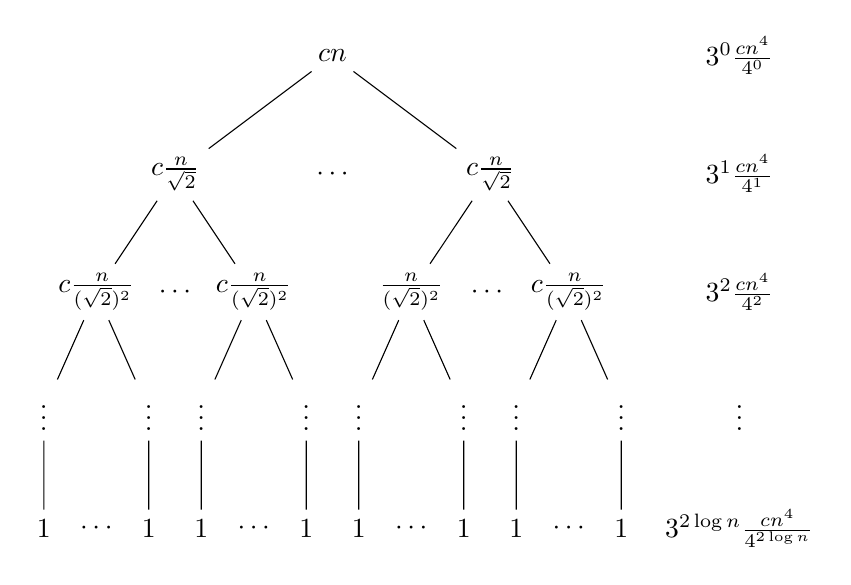
\begin{tikzpicture}[level/.style={sibling distance=40mm/#1}]
\node (z){$cn$}
  child {node (a) {$c\frac{n}{\sqrt{2}}$}
    child {node  (b) {$c\frac{n}{(\sqrt{2})^2}$}
      child {node (b1) {$\vdots$}
       child {node (b11) {$1$}}
      }
      child {node (b2) {$\vdots$}
       child {node (b12) {$1$}}
      }
    }
    child {node (g) {$c\frac{n}{(\sqrt{2})^2}$}
      child {node (g1) {$\vdots$}
       child {node (g11) {$1$}}
      }
      child {node (g2) {$\vdots$}
       child {node (g12) {$1$}}
      }
    }
  }
  child {node  (j) {$c\frac{n}{\sqrt{2}}$}
    child {node (k) {$\frac{n}{(\sqrt{2})^2}$}
      child {node {$\vdots$}
       child {node (k11) {$1$}}
      }
      child {node {$\vdots$}
       child {node (k12) {$1$}}
      }
    }
    child {node (l) {$c\frac{n}{(\sqrt{2})^2}$}
    child {node {$\vdots$}
     child {node (l11) {$1$}}
    }
    child {node (c){$\vdots$}
     child {node (l12) {$1$}
            child [grow=right] {node (r) {$3^{2\log n}\frac{cn^4}{4^{2\log n}}$} edge from parent[draw=none]
              child [grow=up] {node (s) {$\vdots$} edge from parent[draw=none]
                child [grow=up] {node (t) {$3^{2}\frac{cn^4}{4^{2}}$} edge from parent[draw=none]
                  child [grow=up] {node (u) {$3^{1}\frac{cn^4}{4^{1}}$} edge from parent[draw=none]
                   child [grow=up] {node (u) {$3^{0}\frac{cn^4}{4^{0}}$} edge from parent[draw=none]}
                  }
                }
              }
            }
            }
    }
  }
};
\path (b) -- (g) node [midway] {$\cdots$};
\path (a) -- (j) node [midway] {$\cdots$};
\path (k) -- (l) node [midway] {$\cdots$};
\path (b11) -- (b12) node [midway] {$\cdots$};
\path (g11) -- (g12) node [midway] {$\cdots$};
\path (k11) -- (k12) node [midway] {$\cdots$};
\path (l11) -- (l12) node [midway] {$\cdots$};
\end{tikzpicture}
\end{center}

Drawing the recursion tree, there are $3^i$ nodes at level $i$, each doing at most $cn^4/4^i$ work. So the total work at level $i$ is $3^i \frac{cn^4}{4^i}$. Summing over the entire tree we get, 

\[
	\begin{split}
		T(n) &= \sum_{i=0}^{2\log n} 3^i \frac{cn^4}{4^i} \\
		&= cn^4 \sum_{i=0}^{2\log n} (3/4)^i \\
		&< cn^4 \sum_{i=0}^{\infty} (3/4)^i \\
		&< cn^4 \sum_{i=0}^{\infty} (3/4)^i \\
		&< 4cn^4\\
		&= O(n^4)
	\end{split}
\]

The worst case running time is $T(n) = O(n^4)$. Also, $\Theta(1)$ work is done at each leaf, and there are $3^{2 \log n}$ leaves, the total work is at least $\Omega(3^{2 \log n})$. 

\textbf{Master Theorem:} For the recurrence above: \(a=3, \quad b=\sqrt{2}, \quad f(n) = O(n^4)\)  

\[n^{\log_b a} = n^{2 \log_2 3}\]

Since \( f(n) = \Omega(n^{2 \log_2 3+\epsilon})\), where \( \epsilon > 0\), and $\frac{3}{4}n^4 < cn^4$ for any $\frac{3}{4} < c < 1$, from case 3 of the master theorem we get,
\[ T(n) = \Theta(f(n)) = \Theta(n^4)  \]

\problempart % Problem 1c
\( T(n) = 2T\left (\frac{n}{2}\right ) + 5n\log n \) \\

\textbf{Recursion Tree:}

\begin{center}
	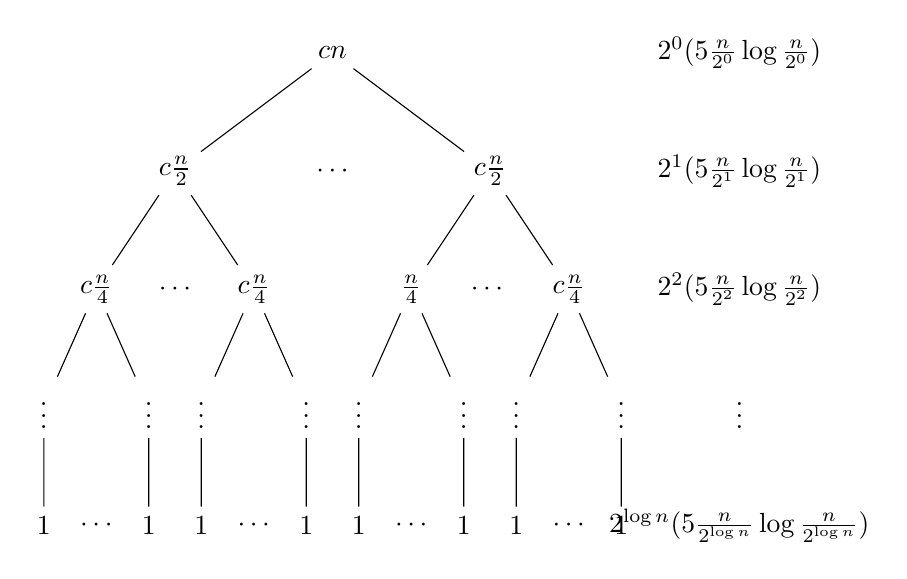
\begin{tikzpicture}[level/.style={sibling distance=40mm/#1}]
\node (z){$cn$}
  child {node (a) {$c\frac{n}{2}$}
    child {node  (b) {$c\frac{n}{4}$}
      child {node (b1) {$\vdots$}
       child {node (b11) {$1$}}
      }
      child {node (b2) {$\vdots$}
       child {node (b12) {$1$}}
      }
    }
    child {node (g) {$c\frac{n}{4}$}
      child {node (g1) {$\vdots$}
       child {node (g11) {$1$}}
      }
      child {node (g2) {$\vdots$}
       child {node (g12) {$1$}}
      }
    }
  }
  child {node  (j) {$c\frac{n}{2}$}
    child {node (k) {$\frac{n}{4}$}
      child {node {$\vdots$}
       child {node (k11) {$1$}}
      }
      child {node {$\vdots$}
       child {node (k12) {$1$}}
      }
    }
    child {node (l) {$c\frac{n}{4}$}
    child {node {$\vdots$}
     child {node (l11) {$1$}}
    }
    child {node (c){$\vdots$}
     child {node (l12) {$1$}
            child [grow=right] {node (r) {$2^{\log n} (5 \frac{n}{2^{\log n}}\log \frac{n}{2^{\log n}})$} edge from parent[draw=none]
              child [grow=up] {node (s) {$\vdots$} edge from parent[draw=none]
                child [grow=up] {node (t) {$2^2 (5 \frac{n}{2^2}\log \frac{n}{2^2})$} edge from parent[draw=none]
                  child [grow=up] {node (u) {$2^1 (5 \frac{n}{2^1}\log \frac{n}{2^1})$} edge from parent[draw=none]
                   child [grow=up] {node (u) {$2^0 (5 \frac{n}{2^0}\log \frac{n}{2^0})$} edge from parent[draw=none]}
                  }
                }
              }
            }
            }
    }
  }
};
\path (b) -- (g) node [midway] {$\cdots$};
\path (a) -- (j) node [midway] {$\cdots$};
\path (k) -- (l) node [midway] {$\cdots$};
\path (b11) -- (b12) node [midway] {$\cdots$};
\path (g11) -- (g12) node [midway] {$\cdots$};
\path (k11) -- (k12) node [midway] {$\cdots$};
\path (l11) -- (l12) node [midway] {$\cdots$};
\end{tikzpicture}
\end{center}

Drawing the recursion tree, there are $2^i$ nodes at level $i$, each doing $5 \frac{n}{2^i}\log \frac{n}{2^i}$ work. So the total work at level $i$ is $2^i (5 \frac{n}{2^i}\log \frac{n}{2^i})$. Summing over the entire tree we get, 

\[
	\begin{split}
		T(n) &= \sum_{i=0}^{\log n} 2^i (5 \frac{n}{2^i}\log \frac{n}{2^i}) \\
		&= \sum_{i=0}^{\log n} 5n (\log n - i)\\
		&= 5n \sum_{j=0}^{\log n} j\\
		&= 5n \log n (\log n - 1)/2 \\
		&= \Theta(n\log^2 n)
	\end{split}
\]

The running time of the algorithm is $T(n) = \Theta(n\log^2 n)$.

\textbf{Master Theorem:} For the recurrence above: \(a=2, \quad b=2, \quad f(n) = 5n\log n\) 

\[n^{\log_b a} = n^{2 \log_2 2} = n\]

Since \( f(n) = \Theta(n^1 \log^1 n)\), from case 2 of the master theorem we get,
\[ T(n) = \Theta(n \log^2 n) \]


\problempart % Problem 1d
\( T(n) = T(n-2) + \Theta(n)\) \\

	Guess that the solution is \( T(n) = O(n^2) \). We choose a function $g(n)$ from the family of functions above. A good candidate is \boldmath \(g(n) = cn^2\) \unboldmath. 
	
	We have to prove using induction that for appropriate constants $c$ and $d$, 
	\[ P(i):= T(n) \leq cn^2\] 
	
	\textbf{Base Case:} \( T(1) = 1 \leq c1^2\). This base case is true when,
	\begin{equation}
	\label{eq:1}
		c\geq 1
	\end{equation}

\textbf{Inductive Step:} Assume P(m) is true, \( \forall m < n \). Then,
\begin{equation}
	\begin{split}
		T(n)  &=  T(n-2) + \Theta(n) \\
			&\leq c(n-2)^2 + \Theta(n) \\
			&\leq cn^2-4cn+4c + \Theta(n)
	\end{split}
\end{equation}

$T(n) = cn^2$, when $\Theta(n) = 4cn - 4c$. Therefore, there exists a value $c$ such that P(n) is true. So it follows by induction that P(n) is true $\forall n$.

\end{problemparts}

\newpage
\problem  % Problem 2

\begin{problemparts}
\problempart % Problem 2a
\problempart % Problem 2b
\problempart % Problem 2c
\end{problemparts}

\newpage
\problem  % Problem 3

\newpage
\problem  % Problem 4

\newpage
\problem  % Problem 5

\begin{problemparts}
\problempart % Problem 5a
\problempart % Problem 5b
\problempart Submit your implementation to {\small\url{alg.mit.edu}}.
\end{problemparts}

\end{problems}

\end{document}
